\textcolor{principal}{\textbf{PROCEDIMIENTO TECNICO PT-UE PARA LA ELABORACION DE TRABAJOS VALUATORIOS QUE PERMITAN DICTAMINAR EL VALOR DEL PATRIMONIO DE LAS UNIDADES ECONOMICAS.}}\\

1.- \textit{Introducci\'on (...)}\\

\textit{Premisas a la valuaci\'on de unidades econ\'omicas}\\
\begin{enumerate}[\indent\itshape a)]
\item \textit{Se analizan las unidades econ\'omicas como negocio en marcha} 
\item \textit{Se podr\'a valuar la unidad econ\'omica como un todo o las partes que la conforman}
\item \textit{Solamente pueden valuar unidades econ\'omicas peritos que cuenten con la especialidad valuatoria en negocios}
\item \textit{Se estima el valor comercial de unidades econ\'omicas}
\item \textit{Este procedimiento cumple en su desarrollo con los ocho pasos del proceso valuatorio establecidos en las metodolog\'ias y criterios de car\'acter t\'ecnico, considerando en todos los casos que existe una solicitud previa de trabajo valuatorio y se ha cumplido con el primer paso que consiste en la ``recepci\'on de solicitud''}
\item \textit{Todos los t\'erminos utilizados en este procedimiento se apegan al Glosario de T\'erminos de Valuaci\'on de Bienes Nacionales que emite el INDAABIN}
\item \textit{Todos los componentes y las acciones consideradas en este procedimiento, han sido incorporadas, vigilando que se apeguen al marco legal vigente}
\item \textit{La vigencia legal de los trabajos valuatorios elaborados bajo este procedimiento t\'ecnico, considera las condiciones f\'isicas, t\'ecnicas, econ\'omicas, pol\'iticas y sociales imperantes a la fecha de valores (...)} 
\end{enumerate}

\textit{\textcolor{principal}{1.4.14. Negocio en marcha}.- Es la entidad comercial que contin\'ua en operaci\'on en el futuro previsible. Por lo tanto, se supone que la empresa genera utilidades y que no tiene la intenci\'on ni la necesidad de liquidar o de reducir materialmente la escala de sus operaciones. Los negocios en marcha pueden valuarse mediante el enfoque basado en los costos, el enfoque de ingreso, o mediante el enfoque de comparativo de mercado.}\\

\textit{\textcolor{principal}{1.4.15. Unidad econ\'omica}.- Es un negocio con actividad econ\'omica realizada con el fin de obtener una ganancia, lucro o utilidad; se constituye por un conjunto de activos fijos (terrenos, construcciones, instalaciones, maquinaria, mobiliario y equipo), vinculados a activos intangibles e integrados conforme a un conjunto de tecnolog\'ias que le permiten producir bienes o prestar servicios en condiciones est\'andares de calidad y costo. A diferencia del negocio en marcha, la unidad econ\'omica puede tener o no utilidades; por lo tanto puede valuarse para operaci\'on continua o para liquidaci\'on. (...)}\\

\textit{\textcolor{principal}{1.4.19. Valor como negocio en marcha}.- El valor de una empresa que continua en operaci\'on en el futuro como un todo, sujeto a la utilidad o servicio potencial adecuado de la empresa, con todos sus activos y pasivos, plusval\'ia y potencialidades. Si la empresa es propietaria de las instalaciones que utiliza, \'estas forman parte del valor como negocio en marcha. El concepto implica la valuaci\'on de la empresa en operaci\'on continua.}\\

\textit{\textcolor{principal}{1.4.20. Valor de la unidad econ\'omica como negocio en marcha}.- Es el valor presente de los beneficios futuros esperados de la operaci\'on y desarrollo de la unidad econ\'omica atendiendo a posibles escenarios que toman en cuenta su ubicaci\'on, posici\'on tecnol\'ogica, capacidad instalada, vida \'util consumida, estado de conservaci\'on, potencial de ampliaci\'on y reconversi\'on, demanda de los bienes y/o servicios que produce y disponibilidad de los insumos, dentro de un horizonte de valuaci\'on y en el contexto y perspectivas de la econom\'ia en que se desempe\~na. Existir\'an tantos valores de la unidad econ\'omica como negocio en marcha como escenarios factibles puedan ser planteados. El valor de la unidad econ\'omica como negocio en marcha puede utilizarse para determinar el valor conclusivo de acuerdo al Uso, Prop\'osito y Finalidad del aval\'uo. (...)}\\

\textit{\textcolor{principal}{2.7.3. Evaluaci\'on financiera}.- Una vez que se ha determinado el flujo de efectivo libre, se debe definir la tasa de descuento bajo la cual \'este se ha de descontar a valor presente; para ello el valuador de bienes nacionales debe definir la tasa de descuento de acuerdo al objetivo del estudio, utilizando distintos m\'etodos financieros generalmente aceptados, como pueden ser: el Modelo para la Valoraci\'on de los Activos de Capital (CAPM, por sus siglas en ingl\'es), Teor\'ia de Fijaci\'on de Precios por Arbitraje, el Costo de Capital Promedio Ponderado (CPC o WACC de sus siglas en ingl\'es1), Costo del Capital por Comparables de Negocios del mismo Sector, entre otros.}\\
\textit{O bien, el valuador de bienes nacionales puede referirse al procedimiento t\'ecnico PT-TD para la obtenci\'on de tasas de descuento.}\\
\textit{Al final del horizonte de valuaci\'on se debe establecer el valor residual del negocio, considerando en algunos casos un valor continuo del negocio, asumiendo su operaci\'on a perpetuidad, o en otros, considerando el valor de rescate de los activos menos los costos de cierre de la unidad econ\'omica. El valor residual se aplica siempre y cuando la naturaleza de la unidad econ\'omica lo requiera y debe determinarse mediante principios financieros generalmente aceptados.}\\

\textit{\textcolor{principal}{2.7.4. Valor de la unidad econ\'omica}.- El resultado obtenido mediante el modelo financiero es el valor presente neto, el cual representa el valor del negocio.}\\
\textit{A partir del valor del negocio, se determina el valor de la unidad econ\'omica restando el valor de los pasivos financieros (deuda con bancos, proveedores con costo, deuda subordinada, acciones preferentes, entre otros), sumando el valor de los activos circulantes l\'iquidos o disponibles (normalmente caja e inversiones temporales y en algunos casos cuentas de inventarios no considerados en los flujos de efectivo) y de los bienes no operativos (bienes no utilizados en la operaci\'on de la unidad econ\'omica), y por otro lado restando los pasivos contingentes (ambientales, laborales, legales, entre otros). Este proceso se muestra de manera esquem\'atica a trav\'es de la siguiente figura:}\\

\begin{figure}[H]
\centering
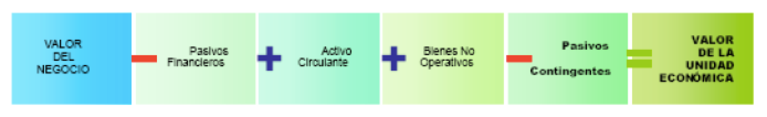
\includegraphics[width=10cm]{\rutaValuatex/sistema/imagenes/pt-ue}
\end{figure}

\textit{\textcolor{principal}{2.8. Estimaci\'on final del valor}.- El valuador de bienes nacionales de negocios en marcha, debe estimar el valor de la unidad econ\'omica como negocio en marcha en funci\'on del Uso, Prop\'osito y Finalidad del trabajo y dictamen valuatorio. (...)''}\\

